\chapter{Further work on the model}
\label{secondPhaseOfModelingCyberInsurance} 

So far our model have only considered the affects from direct connections. Now we are introducing a way of analyzing how network formation will  be affected from indirect connections. 

In the previous models the utility equation for each node have only been affected by direct variables such as $\beta$. In a real world scenario a node will be strongly affected by network externalities. Our idea is based on the paper from Jackson and Wolinsky \cite{jackson1996strategic} and a network formation game in \cite{jackson2005survey}. 

\section{The connection game}
We consider a connection game which reflects not only the benefit from establishing connections to other people, but also the benefits from indirect connections. Meaning, in addition to the benefit from the direct connection, a node will also benefit from "a friend of a friend", although the benefit will be a factor lower than the direct connection, also "friends of a friend of a friend" will generate benefit and so forth. The payoff will be calculated relative to the distance between different nodes.


\begin{figure}[h]
\centering
  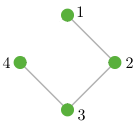
\includegraphics[width=0.2\linewidth]{../Figures/connectionGame.png}
  \caption{\label{fig:connectionGame} Four nodes interconnected with each other.}
\end{figure}
For instance, node 1 in the network depicted in figure \ref{fig:connectionGame}, will benefit $\beta$ from node 2, $\beta^{2}$ from node 3 and $\beta^{3}$ from node 4. The benefit will decrease relative to the shortest path between two nodes as long as $\beta < 1$. Hence the payoff a node receives from the network equals: 

\begin{equation}
\sum_{j\neq i}^{} \beta_{ij}^{d(ij)} - \sum_{j:ij\in g}^{} {I_{l}}_{ij}, 
\label{connecetionGame}
\end{equation}

where $d(ij)$ represents the shortest path between node $i $ and node $j $, and ${I_{l}}_{ij}$ represents node i's cost of insuring a link between the two nodes. To simplify the model we choose a symmetric connection process where $\beta$ and $I_{l}$ is set to a fixed global value. 

To analyze the different outcomes of the game, one might consider making the network as efficient as possible or focus on creating a stable network. An efficient network means ending up with a network which generates the most total value for the players. Intuitively, this network is preferable if it is stable. However, as we shall see there might be some conflict areas between efficiency and stability. 

The paper from \cite{jackson1996strategic} showed that the following propositions for analyzing the game as an efficient network structure:
\begin{enumerate}
\item \textit{a complete graph $g^N$ if $I_{l}<\beta - \beta^2$,}
\item \textit{a star encompassing every node if $\beta - \beta^2 < i_{l} < \beta + \frac{(N-2)}{2}\beta^2$,}
\item \textit{no links if $\beta + \frac{(N-2)}{2}\beta^2 < I_{l}$.}
\end{enumerate}

Generally it means that when the cost of insuring a link is low, it would be more beneficial to have a direct connection to a node than indirectly benefiting from it. When the insurance cost is high, it would not be more beneficial not to establish any connections at all.
The most efficient structure is created in the intermediate cost of insuring links, and ends up in a star structure which encompasses every node. A star structure have the characteristics of minimizing the average path length and uses only a minimal number of links. Indisputable this structure provides the highest overall payoff for the network, however, this network is not stable.
The reason is because the center node of the star will bear the cost of insuring every link connected, which generates a huge cost compared to the other nodes. This scenario is quite unfair, since the center node generates a great deal of network externalities for the other nodes, without being compensated. Hence a number of connections to the center node will not be pairwise stable, and the network will not be stable. 

The conditions has to be changed in order to met the requirements for stability, Jackson and Wolinsky presents the following proposition:

\begin{enumerate}

\item \textit{a pairwise stable network consists of at most one (non-empty) component,}
\item \textit{if $I_{l}<\beta - \beta^2$, the unique pairwise stable network will be a complete graph $g^N$, }
\item \textit{if $\beta - \beta^2 < I_{l} < \beta $, a star encompassing every node will be pairwise stable, although not unique,}
\item \textit{if $\beta < I_{l}$, any pairwise stable network which is nonempty is such that each player has at least two links and thus be inefficient. }
\end{enumerate}

As we can see, the conditions for high and low insurance cost is similar to the previous outcome in the efficient network structure. In addition, the case of intermediate insurance cost will become a stable network, since every new link connected will result in a higher payoff, due to $I_{l} < \beta$. However, it should be noticed that it would be more beneficial for a node to operate at a leaf node in the network, instead of being a center node, due to the cost of insuring each new link. In a perfect star structure, a leaf node will only have to insure the node to the center node, and will benefit indirectly for each node connected to the center node. The center node will benefit from each new connection, however, the payoff will only be $\beta - I{l}$ for each connection. Therefore it is desirable to be a leaf node. 

To solve the problem, one has to compensate the center node for the extra cost of creating network externalities. As described in the previous model considering bulk insurance discount, the insurance company could implement a bonus which lowers the cost for each new connection. This would lower the extra cost for the center node significantly, as it is expected that the number of nodes might be high and therefor result in a significant discount. 
Using the discount calculation from previous models, we end up with the following equation for the star topology:

\begin{equation}
\beta-\beta^2<\frac{i_{l}}{i+1}< \beta
\end{equation}



where $i $ is represent the number of connections a node have established. 

Although this enhancement ensures that the cost for the center node is lowered, it does not guarantee that the center node is fully compensated. To accomplish this, the insurance companies have to directly compensate the center nodes. As described earlier a star topology will create a super critical payoff, and a star topology would be beneficial for the insurance companies. Hence the insurance companies will have incentive to compensate the center nodes additionally to enable the star structure to be generated. 

\chapter{Model from Bohme}


Our model now includes a way of analyzing indirect connectivity among nodes. Inspired by the paper from \cite{danezis2006network} we are now expanding the model to look how network formation works when the nodes have a option to include uninsured nodes in their network. Although the paper tries to observe suseptibility to sybil attacks in peer-to-peer networks, their approach on network formation is related to our insurance network. They propose a network formation game consisting of "friends" and "strangers", which is similar to "insured" vs "non-insured" nodes. 
In a peer-to-peer network the peers selfishly tries to fulfill their communitaction needs, by establishing connections to friends or indirectly via strangers. This is similar to how companies selfishly choose to connect to other nodes with the goal of increasing their utility as much as possible. 

In \cite{danezis2006network} the formation game shows how nodes routes messages between each other. The special case here is that a node does not have enough links to directly connect to everyone. We change the game variables to fit to our model, and the setup for the game is as follows:

\begin{enumerate}

\item There are a set of $N nodes$ which are to be connected in a graph.
\item Each node, $n$ has a set for friends (insured nodes) $F_{n}$ which he want to connect to. The friendship is symmetric.
\item Each node also has a \textit{link budget}, $L_{n}$ which specifies the maximum number of links a node can establish directly to friends. It is also assumed that $L_{n}<F_{n}$. Additionally, if a link is established both nodes will decrease their link budget.
\item Given a graph of links between nodes the utility of each node is calculated using the negative sum of the length of the shortest path to all it friends. Negative sum yields higher utility as the different path lengths decreases.
\end{enumerate}

The goal is obviously to increase the utility. To accomplish this one has to communicate with friends using a minimum number of hoops. If $L_{n}=<F_{n}$ the game would have been a straightforward dominant strategy, where insured nodes only chose to connect to other insured nodes. Hence every node would receive the maximum utility. In the scenario of peer-to-peer network it is easy to understand that one cannot have direct links to every friend on a scale free network, e.g. the Internet, hence $L_{n}<F_{n}$ makes perfect sense. It is also reasonable to take the same assumption  for the insurance market, since one might not have the resources to insure every connection needed, i.e. the link budget $I_{n} < F_{n}$. Hence the nodes might take the risk of connection to non-insured nodes, since the cost of connecting to this node is free.

The graph is created by a pseudo-random selection of a possible link between two nodes. If the utility increases or is stable for both, the link is created and each node decreases their link budget by one.

 
\cite{danezis2006network} proposes two random games which interpret that nodes might have to take the risk of connecting to non-insured nodes.
\begin{enumerate}
\item Random model: Every node in the network initiate a set for friendships with other nodes, denoted $F$. All nodes have the same link budget $L<F$. 
\item Unbalanced Random Mode. The same friendship graph as in the random model is created. However one of the nodes have a significantly larger link budget $(L_{0} > 2 F)$
\end{enumerate}

The first model does not result in any Nash equilibrium, it is believed that every node is eager to use their whole link budget in order to create direct connections to as many insured nodes as possible. In order to reach the rest of the insured nodes, they rely on indirect connectivity via the established connections.

The unbalanced model results in a scenario where the insured nodes still wishes to connect to other insured nodes. The reason for this is claimed to be that the average shortest path in a scale-free graph is $O(log N)$, and the probability that another node, insured or not insured, is closer to to a node is roughly the same. Which means that on average an insured node will benefit from connecting to other insured nodes. 
However, if the link budget only allows each node to only establish 1 link (except the one with a large budget), it will emerge a Nash equilibrium which is star with the rich node in the center. If the rich node is a insured node, all the other insured nodes will connect to this node. 

Maa tilpasse konklusjonene her bedre..








